% ----------------------------------------------------------
% SENSITIVITY ANALYSIS
% ----------------------------------------------------------
\section{Grid-Based Sensitivity Analysis}
\label{sec:sensitivity_analysis}

To operationalize the response-surface view of \CWSL{}, we evaluate the metric
across a finite, user-specified grid of candidate cost ratios
$\Rgrid = \{\R_1, \R_2, \ldots, \R_K\}$.
Rather than committing to a single asymmetry assumption, this procedure exposes
how evaluation outcomes vary as $\R{}$ changes, enabling explicit robustness and
stability checks.

This perspective aligns with established principles of sensitivity analysis,
which emphasize understanding how conclusions depend on uncertain assumptions
rather than optimizing parameters in isolation \citep{saltelli2008}.

\subsection{Candidate grid construction}
\label{subsec:grid_construction}

The grid $\Rgrid$ should span the range of cost asymmetries considered plausible
for the application domain.
In practice, $\Rgrid$ is typically chosen as a small set of positive values,
for example $\{0.5, 1.0, 2.0, 3.0\}$ or a denser logarithmic sequence when finer
resolution is required.
The methods discussed here do not rely on any particular spacing or distribution
of grid points; determinism is ensured as long as the grid is fixed.

Importantly, sensitivity analysis does not require that the ``true'' cost ratio
lie exactly on the grid.
The purpose of $\Rgrid$ is not precise estimation, but controlled exploration of
how conclusions change across a range of assumptions.
For this reason, the candidate grid itself should be treated as a governed
artifact, recorded and reported alongside evaluation outputs to ensure
reproducibility and transparency in downstream decision-making.

\subsection{Evaluating the sensitivity curve}
\label{subsec:sensitivity_curve}

For each $\R_k \in \Rgrid$, we compute $\CWSL(\R_k)$ using identical data and
normalization.
The resulting set of pairs
\[
    \{(\R_k, \CWSL(\R_k))\}_{k=1}^{K}
\]
defines a discrete approximation to the continuous response surface discussed in
Section~\ref{sec:response_surface}.

% --- Figure: response surface over the governed grid ---
% ----------------------------------------------------------
% FIGURE: CWSL response surface vs cost ratio R
% ----------------------------------------------------------
\begin{figure}[t]
\centering
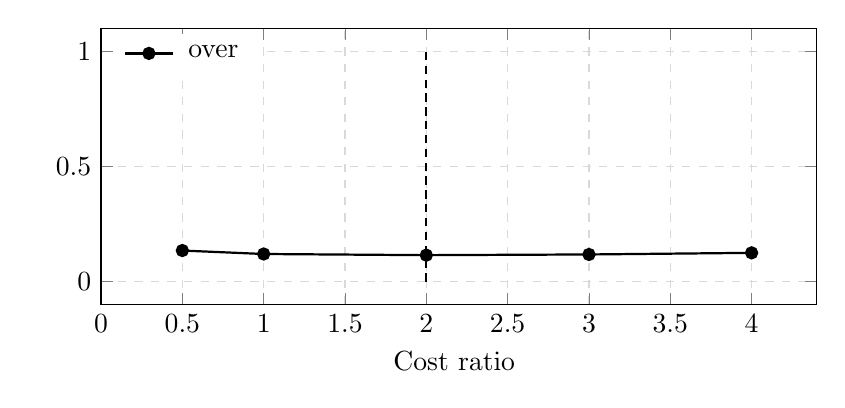
\begin{tikzpicture}
\begin{axis}[
    width=0.88\textwidth,
    height=0.42\textwidth,
    xlabel={Cost ratio $\R{}$},
    ylabel={$\CWSLR{}$},
    xmin=0,
    ymajorgrids=true,
    xmajorgrids=true,
    grid style={dashed,gray!30},
    legend style={draw=none, at={(0.02,0.98)}, anchor=north west},
    legend cell align={left},
]

% --- Placeholder curve (replace with your computed values) ---
% Example grid: R in {0.5, 1.0, 2.0, 3.0, 4.0}
\addplot[
    thick,
    mark=*,
]
coordinates {
    (0.5, 0.135)
    (1.0, 0.120)
    (2.0, 0.115)
    (3.0, 0.118)
    (4.0, 0.125)
};
\addlegendentry{$\CWSLR{}$ over $\Rgrid{}$}

% --- Optional: show calibrated R* as a vertical marker ---
% Replace 2.0 with your calibrated \Rstar{} value.
\addplot[densely dashed, thick] coordinates {(2.0, 0.0) (2.0, 1.0)};
\node[anchor=south west] at (axis cs:2.0, 0.115) {$\Rstar{}$};

% --- Optional: show a "business-chosen" R as a dotted marker ---
% Uncomment and replace 3.0 with your governed default if desired.
% \addplot[dotted, thick] coordinates {(3.0, 0.0) (3.0, 1.0)};
% \node[anchor=south west] at (axis cs:3.0, 0.118) {$\R{}_{\mathrm{gov}}$};

\end{axis}
\end{tikzpicture}
\caption{
Cost-Weighted Service Loss evaluated across a governed candidate grid
$\Rgrid{}$. Marking $\Rstar{}$ on the response surface makes sensitivity and
stability regions explicit and supports auditable model comparison under cost
asymmetry assumptions.
}
\label{fig:cwsl_response_surface}
\end{figure}

Table~\ref{tab:cwsl_sensitivity} reports the corresponding cost decomposition,
making explicit the realized underbuild and overbuild contributions underlying
the response surface and the selection of $\Rstar{}$.

% --- Table: sensitivity + cost decomposition over the governed grid ---
\input{tables/cwsl_cost_ratio_sensitivity_table}

This sensitivity curve provides more information than a single-point estimate.
In particular, it allows practitioners to:
\begin{itemize}[leftmargin=*]
    \item identify regions where \CWSL{} is relatively insensitive to $\R{}$,
    \item detect ranges of $\R{}$ where evaluation outcomes change rapidly,
    \item compare competing forecasts under consistent cost-assumption stress tests.
\end{itemize}

Because the curve is computed from historical residuals alone, it reflects
realized behavior rather than hypothetical model properties.

\subsection{Stability and robustness diagnostics}
\label{subsec:stability_diagnostics}

Sensitivity analysis naturally yields diagnostics that support governed use of
asymmetric metrics.
Flat or gently sloped regions of the sensitivity curve indicate that evaluation
results are robust to moderate mis-specification of $\R{}$.
In contrast, steep segments or sharp changes in curvature signal fragility, where
small differences in assumed cost asymmetry may materially alter conclusions.

These diagnostics are particularly important in model comparison.
If two forecasting approaches cross in ranking at different values of $\R{}$, then
any claim of superiority depends implicitly on a narrow range of cost
assumptions.
Grid-based sensitivity analysis makes such dependencies explicit, allowing
decision-makers to assess whether a chosen model is robust to uncertainty in
operational costs.

\subsection{Role of sensitivity analysis in calibration}
\label{subsec:role_in_calibration}

Sensitivity analysis does not, by itself, prescribe a single ``correct'' cost
ratio.
Instead, it provides the context within which calibration rules can be applied.
By first inspecting the response surface, practitioners can ensure that any
selected $\R{}$ lies in a region that is stable, interpretable, and aligned with
operational priorities.

In the following section, we introduce a deterministic calibration rule that
selects a reference cost ratio by balancing historical underbuild and overbuild
costs across the sensitivity curve, leveraging the structure revealed by the
grid-based analysis.